% Created 2018-10-18 Do 19:07
% Intended LaTeX compiler: pdflatex
\documentclass[11pt]{article}
\usepackage[utf8]{inputenc}
\usepackage[T1]{fontenc}
\usepackage{graphicx}
\usepackage{grffile}
\usepackage{longtable}
\usepackage{wrapfig}
\usepackage{rotating}
\usepackage[normalem]{ulem}
\usepackage{amsmath}
\usepackage{textcomp}
\usepackage{amssymb}
\usepackage{capt-of}
\usepackage{hyperref}
\usepackage{minted}
\usepackage{float}
\author{Nikolai Weidt}
\date{\today}
\title{Calcback}
\hypersetup{
 pdfauthor={Nikolai Weidt},
 pdftitle={Calcback},
 pdfkeywords={},
 pdfsubject={},
 pdfcreator={Emacs 26.1 (Org mode 9.1.14)}, 
 pdflang={English}}
\begin{document}

\maketitle
\setcounter{tocdepth}{2}
\tableofcontents



\section{What is this?}
\label{sec:orgeff36cd}
This is a script to get the complex refractive index \(n = n * ik\) from the ellipsometric parameters \(\Delta\) and \(\Psi\) I got from a simulation.
The result for 300nm SiO\(_{\text{2}}\) should look like this:

\begin{figure}[htbp]
\centering
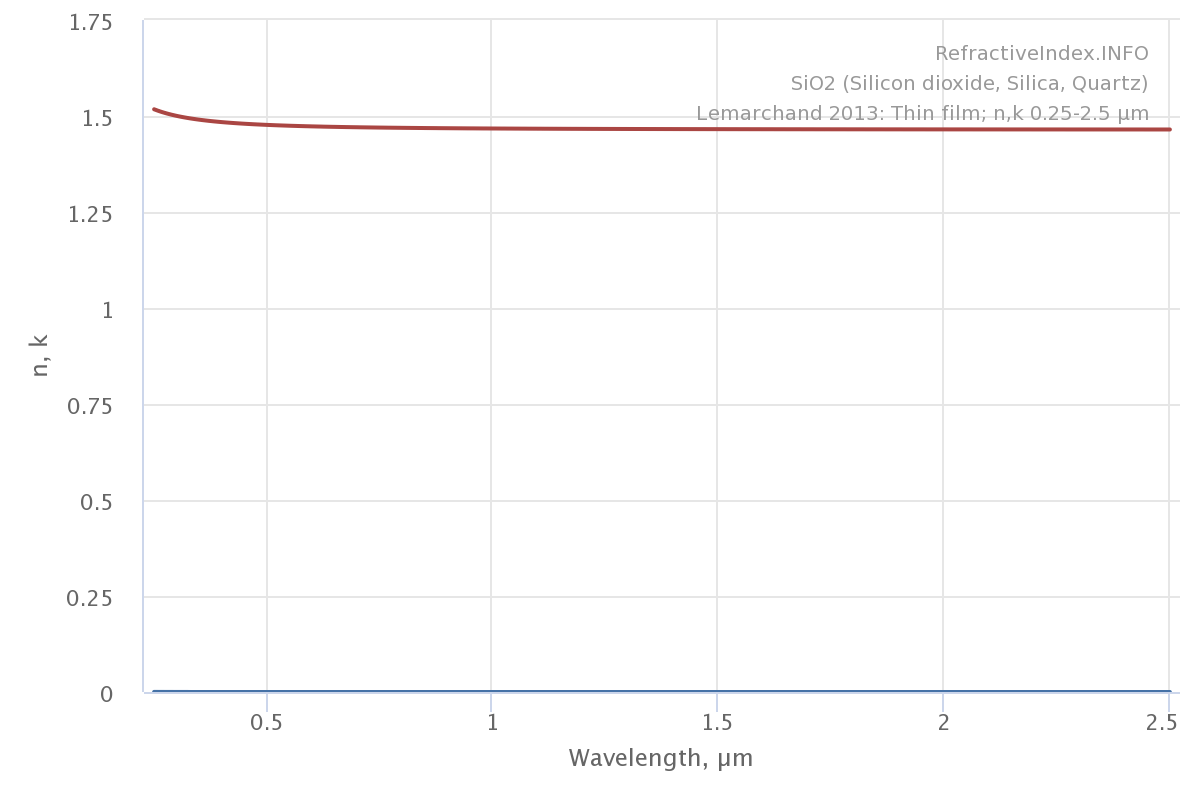
\includegraphics[width=\textwidth]{./RefractiveIndexSiO2.png}
\caption{\label{fig:org424a182}
Refractive index should look like this}
\end{figure}
\section{List of Todos:}
\label{sec:orgca52e7b}

\subsection{{\bfseries\sffamily TODO} Write a loop for all wavelengths after it works for one.}
\label{sec:orga6fb8a8}
\subsection{{\bfseries\sffamily TODO} Then take even more wavelengths (rows)}
\label{sec:org6793dfc}
\section{Imports:}
\label{sec:org8dc8548}
\begin{minted}[]{python}
import numpy as np
import matplotlib
matplotlib.use('Agg')
import matplotlib.pyplot as plt
\end{minted}

\section{Defining some variables:}
\label{sec:orgbad36ae}
Defining some variables for later use:

\begin{minted}[]{python}
CSVFILE = "head300nmSiO2.csv"  # head = only 10 rows of data
phi_i = 70 * np.pi / 180  # converting incident angle from deg (first number) to rad
d_L = 300  # thickness of layer in nm
n_air = 1  # refractive index of air
rerange = 5  # upper limit for real part
imrange = 1  # upper limit for imaginary part
i = 0  # only look at one wavelength (row in csv)
\end{minted}

\section{Read .csv-file:}
\label{sec:org455b840}
Read the values into a two dimensional numpy array as [[lambda,Psi,Delta,n\(_{\text{S}}\), k\(_{\text{S}}\)],\ldots{}] (Skip columns 3 and 4)

\begin{minted}[]{python}
csv = np.loadtxt(CSVFILE, usecols=(0,1,2,5,6),  delimiter=",", skiprows=1)
\end{minted}

The array looks like this:
\begin{minted}[]{python}
csv
\end{minted}

\begin{verbatim}
[[300.          55.2217535   84.37228319   2.6726       3.0375    ]
 [303.          50.11187439  93.3085011    2.7346       3.0381    ]
 [306.          46.35824553  98.43681392   2.7967       3.0368    ]
 [309.          43.50539341 101.18051798   2.8588       3.0334    ]
 [312.          41.29392865 102.19236832   2.9206       3.0279    ]
 [315.          39.48751217 101.93002      2.9822       3.0205    ]
 [318.          37.90308303 100.64846104   3.0435       3.0109    ]
 [321.          36.47640803  98.54577151   3.1042       2.9994    ]
 [324.          35.12615859  95.72242205   3.1644       2.9858    ]]
\end{verbatim}

\section{Calculate \(\rho\)}
\label{sec:org0d3e8ca}
\subsection{Create a matrix containing every possible refractive index (n+ik):}
\label{sec:orgcfc3efe}

Change the last number in the "linspaces" to adjust the resolution.

\begin{minted}[]{python}
lsp_re = np.linspace(1, rerange, 1001)
lsp_im = np.linspace(0.01, imrange, 1001)
re, im = np.meshgrid (lsp_re, lsp_im, copy=False)
n_L = 1j * np.round(im,6) + np.round(re,6)
n_L = n_L.flatten() # create onedimensional array
\end{minted}

This gives the following matrix:
\begin{minted}[]{python}
n_L
\end{minted}

\begin{verbatim}
[1.   +0.01j 1.004+0.01j 1.008+0.01j ... 4.992+1.j   4.996+1.j
 5.   +1.j  ]
\end{verbatim}

\subsection{Calculate \(\rho\):}
\label{sec:org9c8511b}
\subsubsection{First we define some functions:}
\label{sec:org9087c96}
\begin{enumerate}
\item Snell's Law to calculate the refractive angles:
\label{sec:orgc9c8d03}
Phi is the incident angle for the layer, n1 and n2 are refractive indices of first and second medium. Returns the angle of refraction.

\begin{figure}[H]
\centering
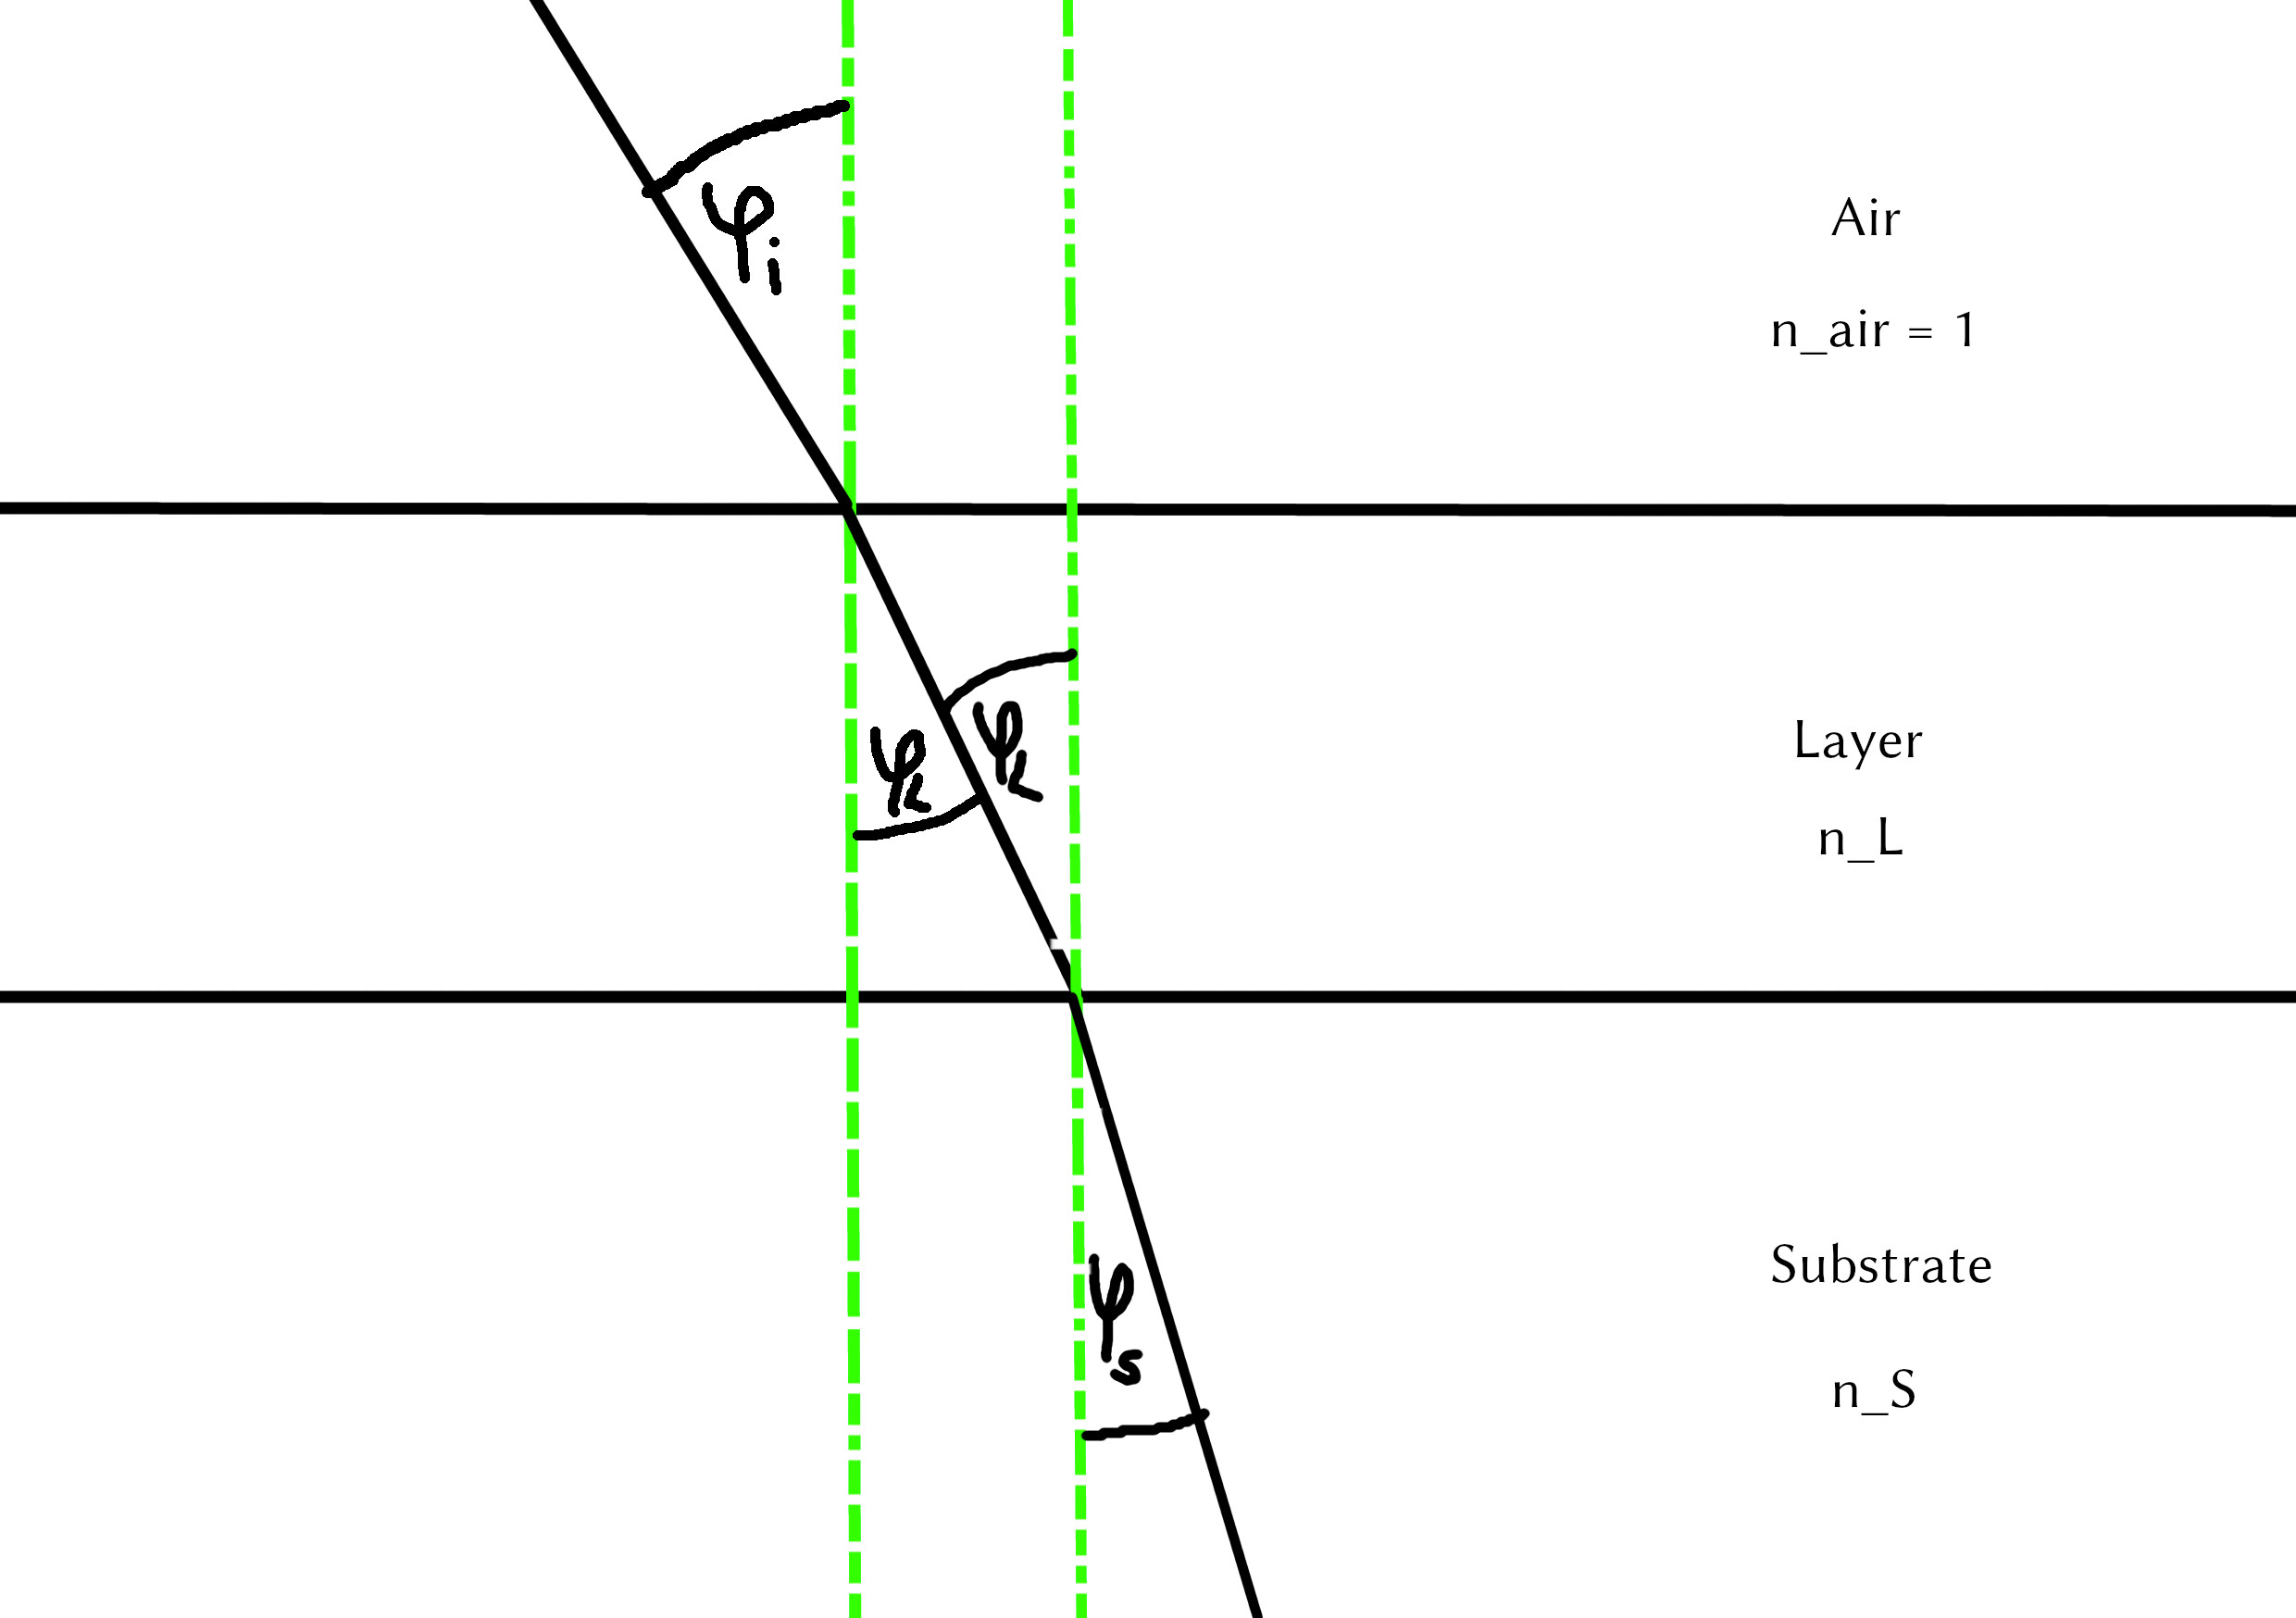
\includegraphics[width=\textwidth]{./snell.jpg}
\caption{\label{fig:orga38d5d6}
Snell's Law}
\end{figure}
\begin{minted}[]{python}
def snell(phi, n1, n2):
  """Calculates the refractive angle, parameters are incident angle phi, refractive index of first medium n1 and of second medium n2"""
  phi_ref = np.arcsin((n1/n2)*np.sin(phi))
  return phi_ref
\end{minted}


\item Calculate r\(_{\text{p}}\) and r\(_{\text{s}}\) with Fresnel equations:
\label{sec:orgcfb450c}
\begin{minted}[]{python}
def fresnel(n1, phi1, n2, phi2):
    """Takes refractive indices and angles of two layers to calculate the amplitude reflection coefficients"""
    rs = (n1 * np.cos(phi1) - n2 * np.cos(phi2)) / (n1 * np.cos(phi1) + n2 * np.cos(phi2))
    rp = (n2 * np.cos(phi1) - n1 * np.cos(phi2)) / (n2 * np.cos(phi1) + n1 * np.cos(phi2))
    return rs, rp
\end{minted}


\item Calculate \(\rho\) for the layer with eq. 5.2 in Spectroscopic Ellipsometry \citenum{fujiwara2009spectroscopic}:
\label{sec:org0914871}
\begin{minted}[]{python}
def calc_rho(rs_al, rp_al, rs_ls, rp_ls, d, n, phi, lambda_vac, returnbeta=False):
    beta = 2 * np.pi * d * n * np.cos(phi) / lambda_vac
    rp_L = (rp_al + rp_ls * np.exp(-2*1j*beta)) / (1 + rp_al * rp_ls * np.exp(-2 * 1j * beta))
    rs_L = (rs_al + rs_ls * np.exp(-2*1j*beta)) / (1 + rs_al * rs_ls * np.exp(-2 * 1j * beta))
    rho_L = rp_L / rs_L
    return rho_L
\end{minted}
\end{enumerate}


\subsubsection{Then we call these functions one after another to calculate \(\rho\):}
\label{sec:org1a6b621}
Get refractive index of the substrate (n\(_{\text{S}}\)) and lambda from the csv:
\begin{minted}[]{python}
lambda_vac = csv[i][0]
n_S = (csv[i][3] + 1j * csv[i][4])
\end{minted}

Then call the above defined functions
\begin{minted}[]{python}
phi_L = snell(phi_i, n_air, n_L)
phi_S = snell(phi_L, n_L, n_S)
# Fresnel equations:
# air/layer:
rs_al, rp_al = fresnel(n_air, phi_i, n_L, phi_L)
# layer/substrate:
rs_ls, rp_ls = fresnel(n_L, phi_L, n_S, phi_S)

rho_L = calc_rho(rs_al, rp_al, rs_ls, rp_ls, d_L, n_L, phi_L, lambda_vac)
\end{minted}


\subsubsection{Identify the best fitting rho with \(\rho\) = tan(\(\psi\)) * e\(^{\text{i}\Delta}\) :}
\label{sec:org4d0a82d}

\begin{minted}[]{python}
# psi is in our csv-file at index 1, delta at index 2 at row "i" for lambda
psi = csv[i][1] * (np.pi/180)
delta = csv[i][2] * (np.pi/180)
rho_giv = np.tan(psi) * np.exp(1j * delta)
diff = abs(rho_giv - rho_L)  # magnitude of complex number
idx = np.argmin(diff)  # index of the minimum
minimum = diff[idx]
n = n_L[idx]
print("At lambda = ", lambda_vac)
print("the layer has the refractive index n_L = " , n)
\end{minted}

\begin{verbatim}
At lambda =  300.0
the layer has the refractive index n_L =  (1.504+0.10108j)
\end{verbatim}

\section{Plot some things for checking results:}
\label{sec:org95d0a47}

If we use a high resolution, those plots are not showing much, thats why they are only showing the first 10000 values.
\subsection{Plot real and imaginary part of the created n\(_{\text{L}}\) matrix:}
\label{sec:orga3522b1}

Real part is blue, imaginary is red.

\begin{minted}[]{python}
fig = plt.figure()
plt.plot(np.real(n_L[:10000]), c='b')
plt.plot(np.imag(n_L[:10000]), c="r")
plt.savefig('n_L.png')
'./n_L.png'

\end{minted}

\begin{center}
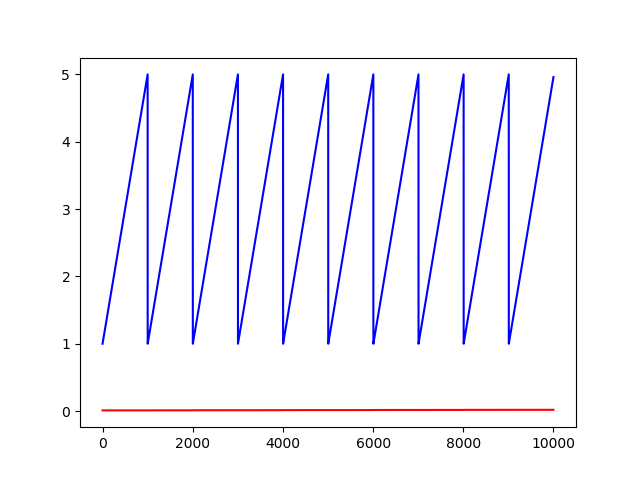
\includegraphics[width=.9\linewidth]{./n_L.png}
\end{center}

\subsection{Plot real and imaginary part of \(\rho_{\text{L}}\)}
\label{sec:org16a36a1}

\begin{minted}[]{python}
fig = plt.figure()
plt.plot(np.real(rho_L), c='b')
plt.plot(np.imag(rho_L), c='r')
plt.savefig('rho_L.png')
"./rho_L.png"
\end{minted}

\begin{center}
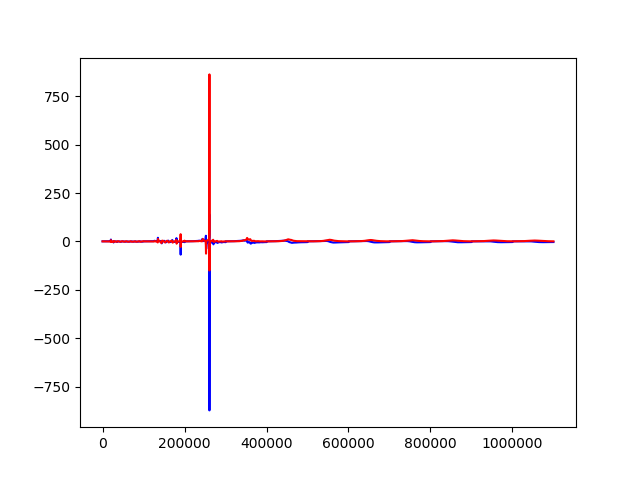
\includegraphics[width=.9\linewidth]{./rho_L.png}
\end{center}

\subsection{Plot of the difference between \(\rho_{\text{L}}\) and the given \(\rho\) and determined minimum:}
\label{sec:org60f690a}

The difference is shown in blue, the red lines show the minimum.

\begin{minted}[]{python}
fig = plt.figure()
plt.axvline(idx, c='r')
plt.axhline(minimum, c='r')
plt.plot(diff[:idx+10000])
plt.savefig('diff.png')
"./diff.png"
\end{minted}

\begin{center}
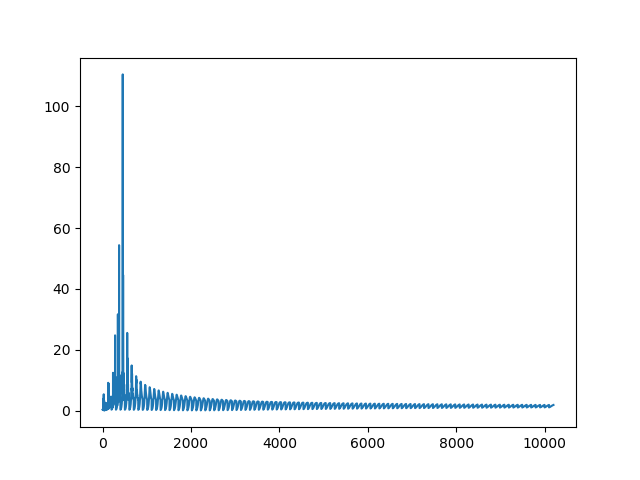
\includegraphics[width=.9\linewidth]{./diff.png}
\end{center}

\subsection{Plot refractive angle phi\(_{\text{L}}\) and n\(_{\text{L}}\):}
\label{sec:org90ebbe5}

n\(_{\text{L}}\) is shown in green, real part of phi\(_{\text{L}}\) in blue, imaginary in red. 
A relation between these should be visible.

\begin{minted}[]{python}
fig = plt.figure()
plt.plot(np.real(phi_L[:5000]), 'b')
plt.plot(np.imag(phi_L[:5000]), 'r')
plt.plot(np.real(n_L[:5000]), c='g')
plt.savefig('phi_L.png')
"phi_L.png"
\end{minted}

\begin{center}
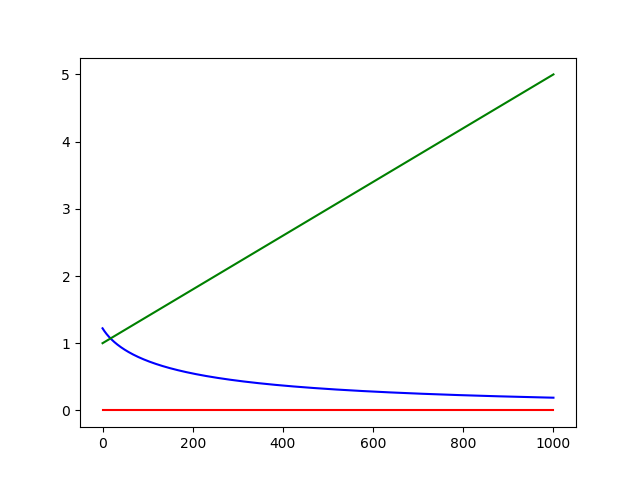
\includegraphics[width=.9\linewidth]{phi_L.png}
\end{center}


\section{Testing:}
\label{sec:orga454f24}

Testing with constant n\(_{\text{L}}\), phi\(_{\text{i}}\) at i=0
\begin{minted}[]{python}
[("n_L[0]",n_L[0]),("phi_i",phi_i)]
\end{minted}

\subsection{snell():}
\label{sec:orgff17aca}

\begin{minted}[]{python}
phi_Ltest = snell(phi_i, n_air, n_L[0])
phi_Ltest
\end{minted}
should be: (1.220429-0.02737074 i)

\begin{minted}[]{python}
("n_S",n_S)
\end{minted}

\begin{minted}[]{python}
phi_Stest = snell(1.220429-0.0273775j,n_L[0],n_S)
phi_Stest
\end{minted}

\begin{center}
\begin{tabular}{l}
0.15167146706201226-0.1754944190504326j\\
\end{tabular}
\end{center}
should be: (0.151671-0.175494i)



\subsection{fresnel():}
\label{sec:orgb3471e2}

rs\(_{\text{al}}\), rp\(_{\text{al}}\) = fresnel(n\(_{\text{air}}\), phi\(_{\text{i}}\), n\(_{\text{L}}\), phi\(_{\text{L}}\))

rs\(_{\text{ls}}\), rp\(_{\text{ls}}\) = fresnel(n\(_{\text{L}}\), phi\(_{\text{L}}\), n\(_{\text{S}}\), phi\(_{\text{S}}\))

\begin{minted}[]{python}
rs_altest, rp_altest = fresnel(n_air, phi_i, n_L[0], phi_Ltest)
rs_altest
\end{minted}
should be: (-0.003398-0.04239i)
\begin{minted}[]{python}
rp_altest
\end{minted}
should be: 

\begin{minted}[]{python}
rs_lstest, rp_lstest = fresnel(n_L[0], phi_Ltest, n_S, phi_Stest)
rs_lstest
\end{minted}

\begin{minted}[]{python}
rp_lstest
\end{minted}

\subsection{calc\(_{\text{rho}}\)():}
\label{sec:orge4ecc23}

rho\(_{\text{L}}\) = calc\(_{\text{rho}}\)(rs\(_{\text{al}}\), rp\(_{\text{al}}\), rs\(_{\text{ls}}\), rp\(_{\text{ls}}\), d\(_{\text{L}}\), n\(_{\text{L}}\), lambda\(_{\text{vac}}\))
 Just copied this from above with beta returned 
\begin{minted}[]{python}
def calc_rhotest(rs_al, rp_al, rs_ls, rp_ls, d, n, phi, lambda_vac):
    beta = 2 * np.pi * d * n * np.cos(phi) / lambda_vac
    rp_L = (rp_al + rp_ls * np.exp(-2*1j*beta)) / (1 + rp_al * rp_ls * np.exp(-2 * 1j * beta))
    rs_L = (rs_al + rs_ls * np.exp(-2*1j*beta)) / (1 + rs_al * rs_ls * np.exp(-2 * 1j * beta))
    rho_L = rp_L / rs_L
    return rho_L, beta
\end{minted}

\begin{minted}[]{python}
rhotest, betatest = calc_rhotest(rs_altest, rp_altest, rs_lstest, rp_lstest, 300, n_L[0], phi_Ltest, lambda_vac)
betatest
\end{minted}
should be: 2.1558487+0.18312240i

\begin{minted}[]{python}
rhotest 
\end{minted}

\section{\bibliography{forschungspraktikum}}
\label{sec:org35c7c1f}
\end{document}